\documentclass[12pt,a4paper]{report}

% Packages for spacing, graphics, math, hyperlinks, bibliography, and code listings
\usepackage{setspace}       % For setting spacing
\usepackage{graphicx}       % For including images
\graphicspath{ {./images/} }
\usepackage{amsmath, amssymb}  % Math packages
\usepackage{hyperref}       % For hyperlinks
\hypersetup{
    colorlinks,
    citecolor=black,
    filecolor=black,
    linkcolor=black,
    urlcolor=black
}
\usepackage{natbib}         % For bibliography formatting
\usepackage{listings}       % For source code listings
\usepackage{xcolor}
\definecolor{codegreen}{rgb}{0,0.6,0}
\definecolor{codegray}{rgb}{0.5,0.5,0.5}
\definecolor{codepurple}{rgb}{0.58,0,0.82}
\definecolor{backcolour}{rgb}{0.95,0.95,0.92}
\lstdefinestyle{mystyle}{
    backgroundcolor=\color{backcolour},   
    commentstyle=\color{codegreen},
    keywordstyle=\color{magenta},
    numberstyle=\tiny\color{codegray},
    stringstyle=\color{codepurple},
    basicstyle=\ttfamily\footnotesize,
    breakatwhitespace=false,         
    breaklines=true,                 
    captionpos=b,                    
    keepspaces=true,                 
    numbers=left,                    
    numbersep=5pt,                  
    showspaces=false,                
    showstringspaces=false,
    showtabs=false,                  
    tabsize=2,
    literate={`}{\textasciigrave}1
}

\lstset{style=mystyle}

\usepackage{microtype}      % For better typography (especially with hyphenation)
\usepackage{etoolbox}
\apptocmd{\thebibliography}{\raggedright}{}{} % Remove underfull \hbox warnings


% Adjust spacing (optional)
\doublespacing

% Define a new command for the supervisor field
\makeatletter
\def\supervisor#1{\gdef\@supervisor{#1}}
\def\@supervisor{}

% Redefine the title page to include a supervisor field
\renewcommand{\maketitle}{
  \begin{titlepage}
    \centering
    % Title
    {\Large \bfseries \@title \par}
    \vskip 1.5cm
    % Author and Supervisor information
    {\large \@author \par}
    \vskip 0.5cm
    {\large \@supervisor \par}
    \vskip 0.5cm
    {\large \@date \par}
    \vfill
    % Optionally include a university logo (uncomment and set path if needed)
    %\includegraphics[width=0.3\textwidth]{university_logo.png}\par
    %{\large University Name\par}
  \end{titlepage}
}
\makeatother

% Title information
\title{Building a Social Media Platform Capable of Scaling to a Million Users Overnight}
\author{Harry Day\\School of Computer Science\\University of Manchester}
\supervisor{Supervisor: Dr. Gareth Henshall}
\date{2025}

\begin{document}

% Generate Title Page
\maketitle

% Abstract
\begin{abstract}
  This is a brief summary of your dissertation. It should outline the research question, methodology, results, and conclusions. 
\end{abstract}

% Table of Contents and Lists of Figures/Tables
\tableofcontents
\listoffigures
\listoftables
\lstlistoflistings

%% These include the actual text
\chapter{Introduction}
\label{cha:intro}

\section{Motivation}
\label{sec:intro-motivation}

\section{Aims and Objectives}
\label{sec:intro-aims}

\section{Scope and Limitations}
\label{sec:intro-scope}

\section{Dissertation Structure}
\label{sec:intro-structure}

\chapter{Background}
\label{cha:background}

\section{The Growth of Social Media}
In recent years, social media has become a cornerstone of modern life with 2.19 billion active users on Facebook in 2018 \citep{saha2019impact}. Emerging adults spend approximately 6 hours using social media daily and frequently use multiple platforms simultaneously \citep{vannucci2019use}.
In contemporary life, ``we draw on the benefits of the ubiquitous networks which provide unparalleled opportunities of economic as well as cultural growth'' \citep{hruska2020use}.
Some social media platforms cater to specific demographics, such as LinkedIn, which targets professionals across every industry.
Despite being a professional network, LinkedIn falls flat at serving the needs of unique demographics, such as young software engineers and computer science students.
These demographics do not actively engage with professional social networks as their older counterparts \citep{florenthal2012college}. 

\subsection{A New Professional Network for Junior Software Engineers}
Junior software engineers should focus on growing their professional networks and their portfolio of personal projects to best position themselves in a competitive post-COVID job market, with open roles for software engineers down 34\% in 2025 from 2020 \citep{fredsoftware2025}

LinkedIn is motivated to cater to its largest demographic, which, in turn, discourages younger demographics from engaging on the platform.
While highly motivated to break into the software industry, this demographic does not engage with the traditional professional networking giant.

\subsection{Scalability in Social Network}
According to Chakradhar and Raghunathan, scalable computing systems maintain consistent performance under an expanded workload.
Social networks must maintain high performance in user experience while experiencing rapid growth in their user base \citep{pujol2010little}.
For example, Twitter experienced a rapid growth in active users of over 1000\% between 2008 and 2009, which resulted in significant downtime due to the architecture not being designed to scale efficiently at that rate \citep{sakaki2010earthquake}.
Scalability should be a fundamental philosophy from the inception of a design.

\chapter{Design}
\label{cha:design}

\section{Architecture}
\label{sec:design-architecture}
Omni will use a microservices architecture. This enables a highly distributed and scalable system that can respond dynamically to changes in incoming requests.
The approach should make use of common industry standards and technology as well as be portable across cloud providers. The aim is to build Omni cloud-natively so that it could scale exponentially in the case of a "viral" moment.
mni will be primarily designed using the microservices architecture. This enables a highly distributed and scalable system, which is able to respond to changes in incoming requests dynamically. 
The approach should make use of common industry standards and technology as well as be portable across cloud providers. The aim is to build Omni cloud-natively so that it could scale exponentially in the case of a "viral" moment.

\subsection{Kubernetes and Containerisation}
\label{sec:design-system-kubernetes}
Kubernetes is an orchestration tool which enables the management of pods across clusters. A cluster is one or more nodes (physical machines) connected together, possibly across different data centres or even regions, which run workloads.


\begin{figure}[htbp]
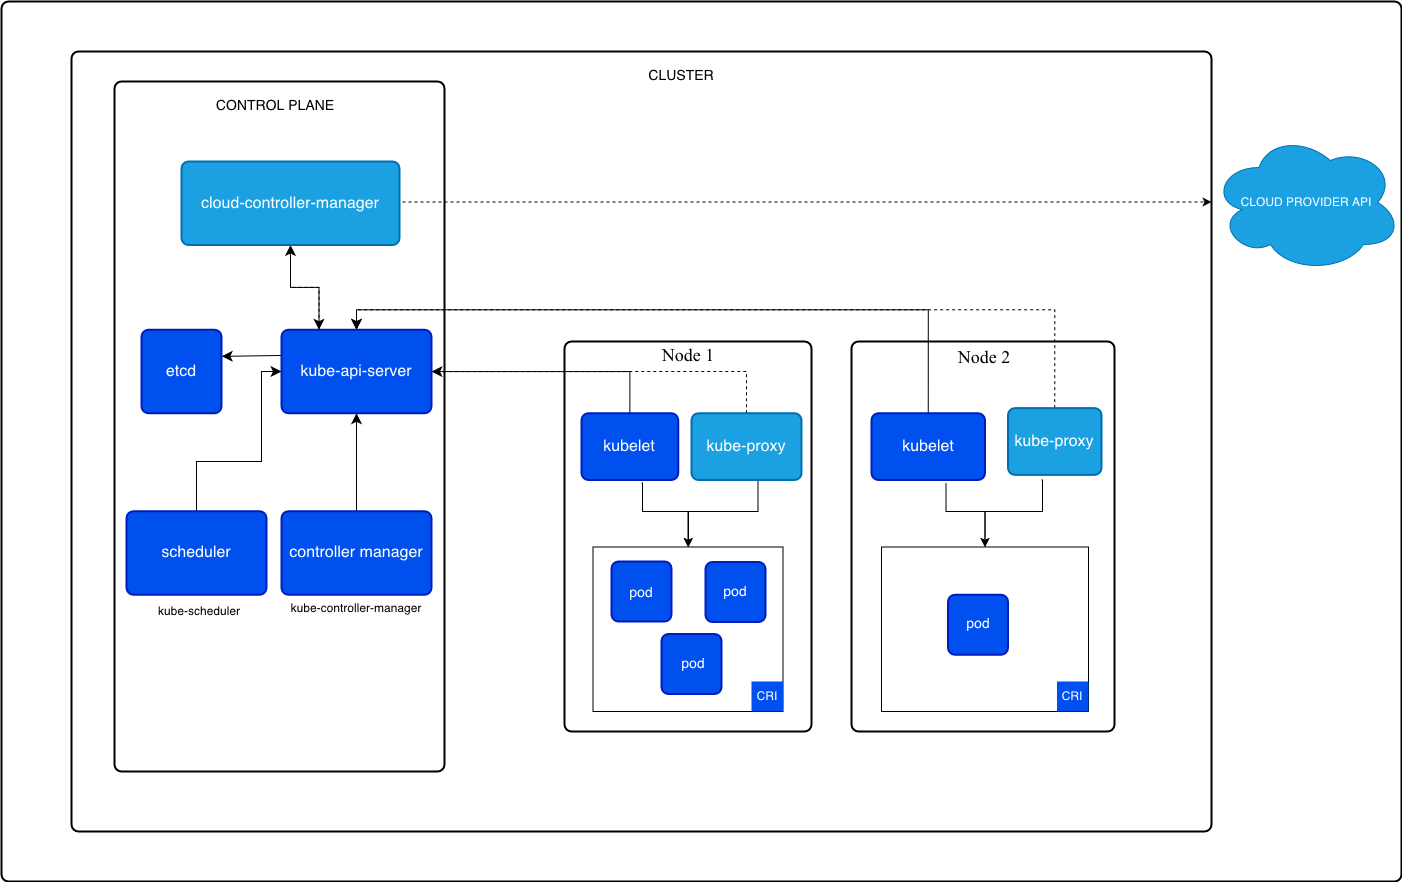
\includegraphics[width=12cm]{k8s-arch.png}
\centering
\caption{Kubernetes Architecture}
\end{figure}

Kubernetes manages the lifecycle of pods using the industry standard health check endpoints \texttt{/healthz}, \texttt{/readyz} and \texttt{/livez}. These endpoints for an application tell Kubernetes whether a pod is running (\texttt{/livez}), ready to respond to requests, possibly checking dependencies like a database (\texttt{/readyz}), and the general health of a pod through \texttt{/healthz}.

Using these endpoints, Kubernetes deployments can monitor the pods (a pod is a running unit usually containing one but sometimes more containers) they have spawned and, if any of them die, for example, if they crash, auto-heal and spawn a replacement.
Deployments can also be configured to scale up the number of pods they run when certain limits are reached. The possibilities are endless, but some common examples could be CPU usage on a particular node or the number of requests received per time period.

This is what makes Kubernetes super powerful. Combining auto-healing and management of ephemeral pods with autoscaling leads to solutions that are highly adaptable to any scenario.
For this reason, Omni will be designed to run natively in Kubernetes. This means that I will need to create containerised applications to run the platform.

Containerisation is the process of modifying an application to run within a container. A container is a self-contained module that can be run without needing to worry about its dependencies or setup. For example, if an application has a dependency on a particular version of Linux with a certain library installed, containerisation will mean that the user running the container can execute the application on any supported OS without needing to worry about the dependencies.

The other added benefit of containers is that the execution environment only needs to contain the compiled binary. Rather than the host machine needing to compile the binary or a CI/CD pipeline creating many binaries for various operating systems, we can use one container, which contains only the compiled binary for the container's OS.

So, for Omni, the application(s) should be containerised and ready for deployment to a Kubernetes cluster in any of the major cloud providers (as well as bare-metal solutions).
Kubernetes is a perfect fit for the microservices architecture described in Section 1: It simplifies the management of individual containers and their lifecycles and provides auto-scaling, rollbacks, service discovery, security and portability. Because of this, Kubernetes is ideal for maintaining scalable and reliable microservice-backed platforms.

\section{Database}
\label{sec:design-system-database}
Omni's database needs to scale horizontally across many machines to handle potentially hundreds of thousands or even millions of users. Database sharding will be needed to ``build scalable, fault-tolerant, and efficient database architectures'' \citep{shethiya2025load}.
In order to accomplish successful database sharding, one of the problems that needs to be solved is how to locate data. Formally:
\begin{quotation} % TODO: Make this not indent weirdly
Given N nodes (where N is sufficiently large), how can a backend locate a specific piece of data whilst preventing a worst case $O(N)$.
\end{quotation}
Ideally, we want data retrieval to be of the order $O(1)$, where a backend knows exactly where to look to find a piece of data that we want to retrieve.

\subsection{Snowflake IDs} 
\label{sec:design-system-database-snowflake}
Luckily, this problem has been solved for us. Engineers at Twitter (now X) faced this same problem and came up with an intuitive solution: snowflake IDs. Snowflake IDs are a type of ID that not only uniquely describes a piece of data but also its locality: where it is stored \citep{2010snowflake}. This enables data to be sharded across many database instances whilst retaining a look-up time with a complexity of $O(1)$.
Snowflake IDs are unique 64-bit integers with the following properties:
\begin{itemize}
    \item The first bit is locked to 0, which ensures that all snowflake IDs are positive. Treating them as signed or unsigned does not matter.
    \item The following 41 bits are dedicated to be a timestamp. This is the time that the ID was created and is based on a custom epoch (rather than the UNIX epoch) to increase the range.
    \item Following the timestamp, each ID has a 10-bit Node ID. This represents the location where a piece of data has been stored.
    \item Finally, we have a 12-bit Sequence ID. This prevents collisions between IDs created for the same Node ID and Timestamp.
\end{itemize}
\ref{tab:snowflake} shows the final structure of the 64-bit Snowflake ID.

\begin{table}[htbp]
\centering
\begin{tabular}{|l|l|l|l|}
\hline
1 bit unused & 41 bit timestamp & 10 bit node id & 12 bit sequence id \\ \hline
\end{tabular}
\caption{Snowflake ID Structure}
\label{tab:snowflake}
\end{table}

Using these Snowflake IDs, it becomes obvious how to store data across many nodes while retaining an efficient retrieval mechanism. A backend only needs to inspect the bits representing the snowflake's node to determine where to route its request. Using 10 bits for this value also allows us to scale up to 1024 nodes, which should be plenty for even the largest social media networks.

When using Snowflake IDs, the key concern is ensuring that only a single object in a given backend can create the IDs and that each backend is assigned a unique Node ID (even if multiple Node IDs are stored in the same database shard). 
This prevents ID collisions during generation, rather than using a 128-bit ID like the one specified in the RFC 4122 UUID specification \citep{rfc4122}.

\subsection{Database Implementation}
A classic SQL database will suit our needs since the data we will store in a social media network is structured, where the relationships between users, posts, and comments are known.
The added flexibility of a NoSQL database, whilst attractive for sharding, is not warranted for such a platform, and a more strict and structured scheme should bring benefits in the long run compared to developer experience and stability.

Given this directive, some natural choices are SQLite and MySQL/MariaDB. They are both simple and robust; however, MySQL/MariaDB is better suited for this particular application with a single (sharded) database. In lightweight/mobile applications, SQLite is the preferred option.

As mentioned above in Section \ref{sec:design-system-database-snowflake}, the database will be sharded so that the load of multiple backends accessing data from the database is balanced across multiple servers. 
This allows databases to be located in separate regions and balances the load across multiple servers.
Another option to balance the load on the database is to use read replicas, where there is one primary node and many read replicas, which are a copy of the primary node.
This setup is perfect for read-heavy applications, as read requests are distributed across the replicas.
It also brings the benefit of higher availability, as all servers have the same database, so if the primary node fails, other nodes can be promoted to receive write requests.
Replication does bring a write bottleneck where only one server can process writes to maintain ACID compliance. 

Overall, sharding is the better option for the Omni platform due to the write bottleneck and the potentially massive amount of data that will be stored in the database.
A future improvement would be to use a hybrid approach, where some things, like the user profile data, which is not expected to receive many writes, are stored in a replicated database, whereas post and comment data is stored in a sharded database to prevent a bottleneck when writing.


\section{Backend}
\label{sec:design-system-backend}
Omni has a couple of requirements for the backend:
\begin{itemize}
    \item The backend needs to be able to service both users interacting with the frontend as well as via an API
    \item The backend must be able to scale to meet the needs of the incoming requests
\end{itemize}
Considering these requirements, the backend must be designed to scale efficiently. A social media platform expects to receive a lot more read requests than write requests.
Splitting the backend into multiple microservices that can scale to demands independently puts the platform in the best position to maintain availability and reliability. 
One way to achieve this is to use separate microservices for read and write requests. This allows us to scale the read service to use many more instances than the write service during periods of high usage. 

By adopting this approach, we can also split other sections of the application into separate microservices.
For example, we could use an authentication service that is only responsible for logging users in and providing them with a JWT token for future requests.
There is no limit to the granularity of the microservices used.
However, there will likely be a limit of diminishing returns where further breaking down microservices does not lead to significant performance improvements compared to the effort spent creating them.

\subsection{Omni Microservices}
\label{sec:design-system-backend-microservices}
Based on the discussion in Section \ref{sec:design-system-backend} above, Omni's backend is split into three different microservices:
\begin{itemize}
    \item OmniRead, which will handle purely read API requests with no side effects
    \item OmniWrite, which will handle any API request that modifies the \\database
    \item OmniAuth, which will handle authenticating a user when they log in as well as provisioning JWT tokens
\end{itemize}

We do not want separate API endpoints for each service. To route requests to the correct microservice, we will use a layer 4 load balancer. Because requests are balanced based on their HTTP method and path (GET requests are for OmniRead, /login requests are for OmniAuth, and everything else is for OmniWrite), a layer 4 load balancer, which operates at the application layer, is preferred over a lower-level layer 7 load balancer, which operates on TCP/UDP packets.

\section{Frontend}
\label{sec:design-system-frontend}

\subsection{UI Design}
\label{sec:design-ui}

\chapter{Implementation}
\label{cha:implementation}

This chapter will describe in detail the technical implementation of the Omni platform.

\section{Configuration}
Configuration is an important part of any production application. It is any data required by the application for it to run.
Configuration may need to change, and it should be able to do so without requiring developers to rebuild the application.
Allowing configuration to be ephemeral enables companies with separate teams that manage a platform's operations to make configuration changes without the need for intervention by a software developer.

Configuration items should be passed to the application via its environment rather than compiled into its binary.
One method for specifying configuration is through a configuration file. This file (normally JSON or YAML) contains key-value pairs of data for the application to consume at start-up.
Some frameworks even enable the file to be monitored for changes so that the most up-to-date values can be used without requiring a restart. 

Another method preferred in Kubernetes and containerised environments is using environment variables.
These are variables set in the bash environment that the application is executed from. The application can then read the values of these variables and use them for its own configuration.

Kubernetes allows environment variables to be specified in the workload manifests for each application.
This means that if the configuration changes, a new manifest can be loaded to bring new pods online with the updated config. Once the new pods are available and responding to requests, the old pods can be scaled down and removed.

\lstinputlisting[language=Go, caption=Example of Parsing Environment Variables, label={lst:go-env}]{code-snippets/go-env-example.go}

The second method will be used as Omni is designed for Kubernetes. To enable the use of environment variables for configuration, an open-source package called \underline{\href{https://github.com/caarlos0/env}{Caarlos0/env}} \nocite{env} will automatically pull these values from the environment (shown in Listing \ref{lst:go-env}).
Defined in the applications are different configuration objects with the required configuration items included, along with some special tags that indicate the name of the related environment variable.
On start-up, a call to the package automatically creates the configuration objects based on the values from the environment. The config objects can then be passed around the application to the sections of code that require them.

\section{Observability}
Logging and observability are vital to the ongoing stability of any production system. ``The distributed nature of microservices also introduces complexity, making  it  challenging  to  ensure  the  reliability,  performance,  and  security  of  the  system'' \citep{chinamanagonda2022observability}.
Clear and consistent logs are crucial for developers to be able to debug faulty platforms quickly. 

Logging is not the only facet of observability. However, metrics and tracing are also key to building a holistic view of a platform's health.
Metrics are the key numerical data points representing a system's health and behaviour over time.
Metrics often include requests per second, latency and CPU usage. These can be easily aggregated, structured, and visualised in top-level dashboards to provide a glanceable overview of how a platform is performing.
They are the first level of reporting an operations team will monitor.

Traces, on the other hand, record the path that requests take through a platform. They often capture the logs each system produces along the way and measure latencies across the system.
Traces are ideal for identifying bottlenecks and pinpointing failures within a larger microservices architecture. Tracing is often handled by a framework called \underline{\href{https://opentelemetry.io}{Open Telemetry}} \nocite{opentel}, a standardised way of collecting and exporting traces from many different applications.
Figure \ref{fig:opentel-overview} shows an overview of the structure of Open Telemetry.

Finally, logs are the lowest level of the three fundamental observability pillars. Logs are immutable, and applications emit timestamped events to process incoming requests.
Developers with a fine-grained understanding of how the system functions best use logs, which are extremely useful for pinpointing the exact line where a system has failed. 

\subsection{Observability in Omni}
In Omni, the Go standard library's structured logger emits logs, allowing each log to contain extra information, such as variables.
The structured logger can output logs in various formats, the most common being text-based (for console logs) and JSON-based (for consumption into an observability pipeline).

\lstinputlisting[language=Go, caption=Example of Structured Logging]{code-snippets/go-logger-example.go}

\begin{figure}[htbp]
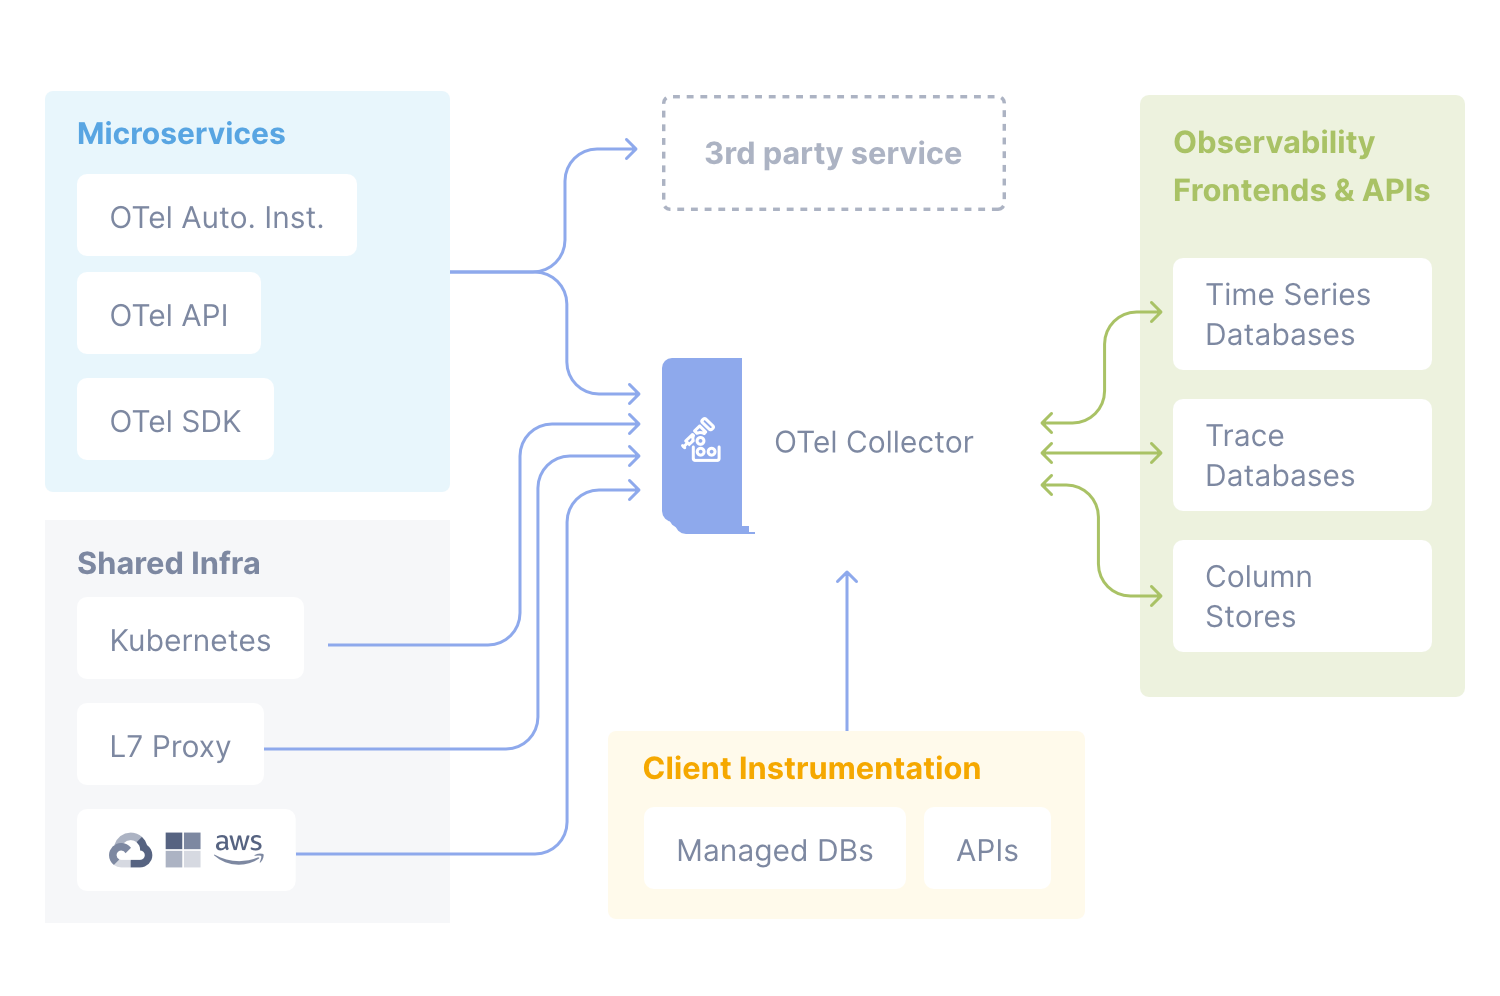
\includegraphics[width=12cm]{otel-diagram.png}
\centering
\caption{An Overview of the Structure of Open Telemetry}
\label{fig:opentel-overview}
\end{figure}

Whilst tracing using a framework such as Open Telemetry would be helpful in a larger production environment, Omni currently only has four microservices.
Tracing has been ignored for the initial product but could easily be retrofitted around the existing logging infrastructure.
An OpenTel Exporter would then consume these traces from many different applications and publish them to a single location, for example, \underline{\href{https://prometheus.io}{Prometheus}} \nocite{prometheus}. 
The Kubernetes cluster provides top-level metrics covering basic needs, while load balancers provide more in-depth metrics, such as requests per second.

\section{Database}
\label{sec:impl-database}
Data is at the centre of every social media platform. The first step in creating Omni should be to build the database in which its data will be stored.
To ensure the database is reproducible on multiple servers (for example, when creating a new database shard), database migrations must be written and applied iteratively on top of one another until the final database structure has been formed. 
There are many tools and libraries for applying database migrations to a database, but since the microservices will be written in GoLang, the GoMigrate tool is a natural fit.

\subsection{Database Tables}
Figure \ref{fig:db-erd} shows the final design of the tables. The Omni platform has two main entities that are easy to see, and a third arises during the implementation.

\begin{figure}[htbp]
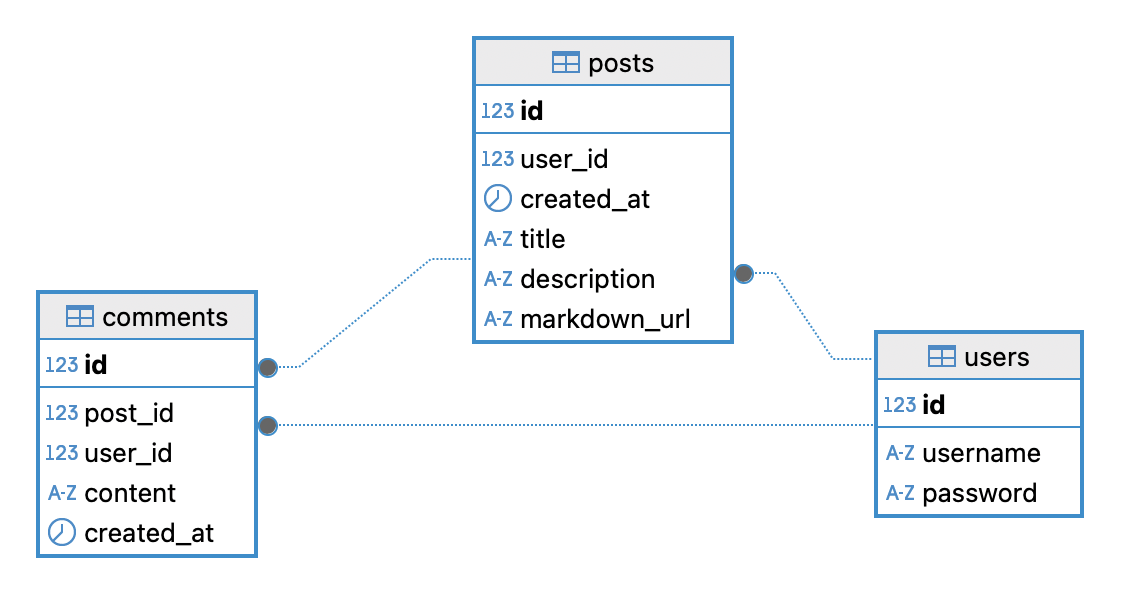
\includegraphics[width=12cm]{db-erd.png}
\centering
\caption{Database Entity Relationship Diagram}
\label{fig:db-erd}
\end{figure}

Information about each user needs to be stored, so a user table is naturally required. This includes any information about the user, such as username and password hash.
In the MVP of Omni, there is not much additional information stored about each user, but we could feasibly expand to store much more data for new features, such as storing a user's birthday.
In the future, if a hybrid approach for database distribution is used, a separate table to hold authentication data may be better to store this on a replicated database cluster rather than a sharded one.

The second easy-to-see table holds information about each post. It must store the creator's ID, title, description, link to the markdown file, timestamp, and more.
Posts will have a one-to-many relationship with users, where one user may create many posts, but each post is always associated with just one user. 

The final table is not as obvious to spot but still crucial: a table to store comments in. Storing this in the posts table does not make sense in a structured SQL database.
Adopting this approach could work in a NoSQL setup, but for popular posts, the document size would grow too big and slow down reading the post for everybody.
By storing the comments in a separate table, we can use pagination in our SQL queries to limit the number of comments we return to a user simultaneously.
This limits the load on the microservices, ensuring they are not overwhelmed by a very popular post with many comments.

\subsection{Discussion on Sharding}
As discussed in Section \ref{sec:design-system-database}, the design of the database and Snowflake IDs enable easy sharding of the database, whilst maintaining fast access times by backend microservices.
A single database has been used to maintain simplicity for the initial implementation and testing of the platform. The only difference this has in the code is that the logic for selecting which database node to retrieve data from is removed (as only one node contains all data).


\section{Backend Microservices}
\label{sec:impl-backend}
This section discusses how the backend microservices were created and how they interact with the broader environment.
Some patterns have been shared across services to enable as much code reuse as possible.

\subsection{Database Access}
\label{sec:impl-backend-db}
All three backend services require some level of database access. OmniAuth and OmniRead require only read access, whereas OmniWrite will read and write data. 

All the applications (currently) interact with the same database, although, as mentioned in Section \ref{sec:design-system-database-implementation}, future improvements could include using separate databases for things like authentication.
Because the database is shared, we can utilise the same database layer in each application, reducing the amount of code we need to write.

\subsubsection{The SQLc Library}
\underline{\href{https://sqlc.dev}{SQLc}} \nocite{sqlc} has been used to generate the database layer automatically.
This code generation library takes as input database migrations and all the queries to be run against the database.
It then compiles these inputs into type-safe code. There are multiple benefits to this approach:
\begin{itemize}
    \item Most of the code generated is boilerplate developers must write by hand or copy from documentation. It does not solve novel problems.
    \item The code generated is type-safe and handles embedding objects from joins for a more traditional object-orientated programming style. 
    \item The compiler flags breaking changes to the database via migrations when the database layer has been regenerated, but the business logic has not yet been modified.
\end{itemize}
Using this approach, SQLc has generated objects for users, posts, and comments, as well as other objects used when retrieving smaller data sections from each table.
Helpfully, the library generates an interface used within the code to access the database and an implementation of the interface for accessing the database.
However, this interface enables developers to write custom implementations, for example, to be used during unit testing. 

\lstinputlisting[language=Go, caption=The Generated GoLang Post Struct]{code-snippets/sqlc-go-models.go}

All the backend services share this database layer as there is no need to write the queries separately for each one, as operations like retrieving a user profile happen in all the services.

\subsubsection{Managing Database URLs}
In order for the services to make calls to the database, they need to know where to send requests.
This is defined by a URL that is passed to each application through the environment, allowing for on-the-fly changes to the configuration without having to rebuild each application. 
The start-up function parses this URL and then creates a database connection using Go's built-in \underline{\href{https://pkg.go.dev/database/sql}{database/SQL}} \nocite{gosqlpkg} package.
Finally, a Querier object (generated by SQLc) is initialised from the database connection object. This is the object which will be passed to each service's business logic so that database requests can be made.

\subsection{Authentication}
Authentication is an important part of any platform. It ensures that users can only access data and perform tasks they are authorised to do. 
Rather than using an authentication library, Omni uses a simple, custom authentication implementation, where users log in using a username and password.

\subsubsection{Sign Up}
\label{sec:impl-auth-signup}
When a user signs up to Omni, they enter a unique username and a password of their choice.
This information is sent to the backend, where the password is hashed using the bcrypt algorithm developed by \citeauthor{provos1999future}.
The GoLang package \underline{\href{https://pkg.go.dev/golang.org/x/crypto/bcrypt}{crypto/bcrypt}} \nocite{gobcryptpkg} handles this. The password hash is then stored in the database along with the rest of the user's details.

\subsubsection{Bcrypt}
The Bcrypt algorithm stores all the information required to verify a password attempt in the hash.

\begin{figure}[htbp]
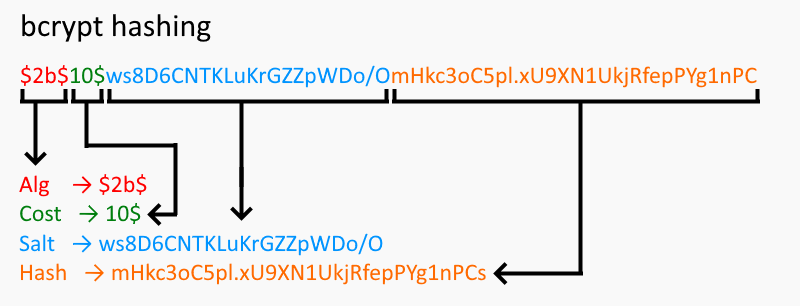
\includegraphics[width=12cm]{bcrypt-parts.png}
\centering
\caption{Sections of the Bcrypt Hash}
\label{fig:bcrypt-parts}
\end{figure}

The first section of the hash contains the algorithm used to create it. Bcrypt uses a version of the Blowfish cypher, denoted by the hash \verb|$2b$|.
The second section is the cost factor used in the algorithm. The default of 10 is used for Omni, but in production, this should be increased to 12 or higher.
Generally, the larger the value of the cost factor, the slower it is to check a password.
While counter-intuitive, this is the desired behaviour, as the slower it is to check a password, the harder it is for a brute-force algorithm to check the most common passwords.
The third section of the hash is the salt used; this is stored as plain text so that it can be used to derive the encryption key for later use.
Finally, the encrypted password is stored as the last part of the hash, which is compared against a potential password.

Checking a password involves deriving the encryption key from the given algorithm, cost factor and salt, using that key to encrypt the given password and then comparing it against the valid password hash. If the hashes match, the password is valid.

\subsubsection{JSON Web Tokens}
JWTs are the industry standard for ongoing authentication. They can contain many standard or custom `claims', which the application uses to determine whether the JWT is valid.
In particular, Omni uses the \verb|exp| and \verb|sub| claims (standing for expires at and subject, respectively). 

After a JWT body is generated, applications hash it using a secret key, which is appended to the JWT to ensure that the body is not modified by anyone other than the authorised applications. 

In subsequent requests to restricted endpoints, clients attach their JWT in the Authorization header of the HTTP request.
The relevant backend, which handles requests to that particular endpoint, can then verify the claims in the JWT.
Based on the subject claim of the JWT, the backend can decide if the client making the request is authorised to do so for the particular action they are performing.
For example, a user can delete a post they have created but cannot delete posts from other users.

\subsection{OmniAuth}
The simplest of the backend services is OmniAuth, which authenticates an existing user to access restricted endpoints.
OmniAuth serves just one endpoint: \verb|POST /api/login|. The handler expects the request to have a JSON body with the fields \verb|username| and \verb|password|. 
The username is used to retrieve the user from the database. When the user does not exist, the endpoint returns a 404 Not Found HTTP error.
The returned data from the database includes the Bcrypt hash of the user's password. 

As mentioned above in Section \ref{sec:impl-auth-signup}, the \underline{\href{https://pkg.go.dev/golang.org/x/crypto/bcrypt}{crypto/bcrypt}} \nocite{gobcryptpkg} package compares the password sent in the request to the hashed password stored in the database.
If the passwords match, the authentication request is valid. If they do not match, the request returns a 401 Unauthorised HTTP error.

Given that the passwords match, OmniAuth will create a JSON Web Token (JWT) that can be used to authenticate the user for subsequent requests to restricted endpoints.

\subsection{OmniRead}
OmniRead, as described in Section \ref{sec:design-system-backend}, is responsible for handling any HTTP Get requests. This allows us to scale read requests separately from the scaling of backend services that handle write requests.
In the initial version of Omni, the data that users need to be able to read is: 
\begin{itemize}
    \item Posts
    \item Users
    \item Comments
\end{itemize}
However, we have more than three endpoints, as users may want to access different data sections differently. For example, a user may want to retrieve all the posts a user has created and the most recent posts by any user. 

All the API endpoints served by OmniRead are unauthorised, meaning that anybody can access them without a JWT token. This simplifies the service regarding the middleware required for each endpoint and its runtime configuration in the Kubernetes environment. 

For some endpoints that could return infinite amounts of data, such as retrieving comments on a post or posts by a particular user, paging is needed.
This ensures that the database and the backend service are not overwhelmed by a denial-of-service attack, where a malicious request can cause the entire service to hang or run out of memory while processing it. 
Paging ensures that the data returned has a maximum size of ten items. Users who wish to see more items can request the next page, which will return the following ten items.

Achieving this paging in the application layer is trivial, but it still leaves the attack vector open. In this scenario, the application layer would still require all the data from the database, even if it only returned a subset to the user. 
Luckily, popular SQL databases already have this paging feature built-in through the \verb|LIMIT| and \verb|OFFSET| keywords.
\verb|LIMIT|, as the name suggests, limits the number of rows of data returned, and \verb|OFFSET| skips the number of rows specified.
For example, with a \verb|LIMIT| of 10 and \verb|OFFSET| of 0, the first 10 rows will be returned. With an \verb|OFFSET| of 10, rows 11-20 are returned. 

\lstinputlisting[language=SQL, caption=Example of SQLc Query with LIMIT and OFFSET]{code-snippets/sql-limit-example.sql}

Other paging strategies also exist. For example, in the context of comments, a user may prefer to page by time, finding all the comments before or after a timestamp.
This paging application is more useful for other applications that use the API, perhaps for research purposes.
In contrast, users interacting with the Omni platform via the website will likely want to read the most recent comments on a post or the highest-rated comments if a liking system is introduced.
The \verb|LIMIT| and \verb|OFFSET| approach is more efficient for these cases when compared to the client specifying a timestamp or other parameter to find comments before or after, with different sorts applied to the query. 

OmniRead returns data in the response body in a JSON format. JSON is the standard format for transmitting data in APIs on the web.
Whilst other more efficient formats exist, such as \underline{\href{https://protobuf.dev}{ProtoBuf}} \nocite{protobuf}, JSON is ubiquitous and well-supported by most languages' standard libraries.
GoLang has powerful, built-in tooling to encode and decode to and from the JSON format into standard GoLang structs.
As part of a set of helper functions for all the backend services, Omni has a helper function that takes an object and an HTTP Response Writer object and writes the JSON encoding of the object to the response along with a 200 Success HTTP code.
This helper function is used across all the backend services to transmit data to the request sender. 

Throughout the OmniRead service (and all the backend services), Omni attempts to reflect as much information as possible through HTTP Status Codes.
Some examples include 200 Success and 201 No Content when requests are successful, with the former indicating there is some returned content in the body of the response, whilst the latter means nothing was returned.
When a request is malformed or otherwise incorrect, status codes in the range 4XX are returned depending on the type of error.
Finally, the service returns 500 Internal Server Error and 503 Service Unavailable errors when the backend encounters errors it cannot recover from, such as the database being down. 

Consumers of the API should be able to use HTTP Status Codes as the first port of call to immediately know if a request was successful, rather than the way that some more modern JavaScript frameworks hide errors inside of 200 Success messages.
The practice of hiding errors inside responses that return with a 200 code can lead to poor error handling and unexpected fatal crashes.

\chapter{Testing and User Feedback}
\label{cha:testing}

Testing is an important facet of any programming. It ensures that the code is functional and free from logical errors.
Test-driven development (TDD) is the practice of writing unit tests before implementing a feature or bug fix, allowing developers to define exactly how a specific function is expected to work given a set of inputs before focusing on how the function achieves the correct outputs.
Defect rates have been shown to decrease by around 50\% when following TDD, compared to a traditional style of testing, where tests are written after the fact \citep{maximilien2003assessing}.

\section{Unit Testing}
Unit tests are a fundamental form of testing for all applications. They are small, focused tests that verify the correctness of individual components of a system.
Each test checks whether a specific function produces the expected outputs, given a set of inputs.
Unit tests are reusable by design, building into a suite of tests that are quick to run over time and ensure regressions do not occur.
Regression tests are particularly valuable as they increase confidence that new changes do not break existing features unexpectedly.
The field of regression testing and minimisation of regression tests is vast.
However, much work has been done to automate the selection of regression tests to keep overall costs (time and energy) down whilst still providing a comprehensive suite of tests which aim to cover as much of the application as possible \citep{wong1997study}. 

Omni utilises unit tests to cover most of the codebase, aiming for code coverage of over 70\% but achieving close to 100\% across the key, testable areas of the codebase (shown in Figure \ref{fig:test-coverage}).

\begin{figure}[htbp]
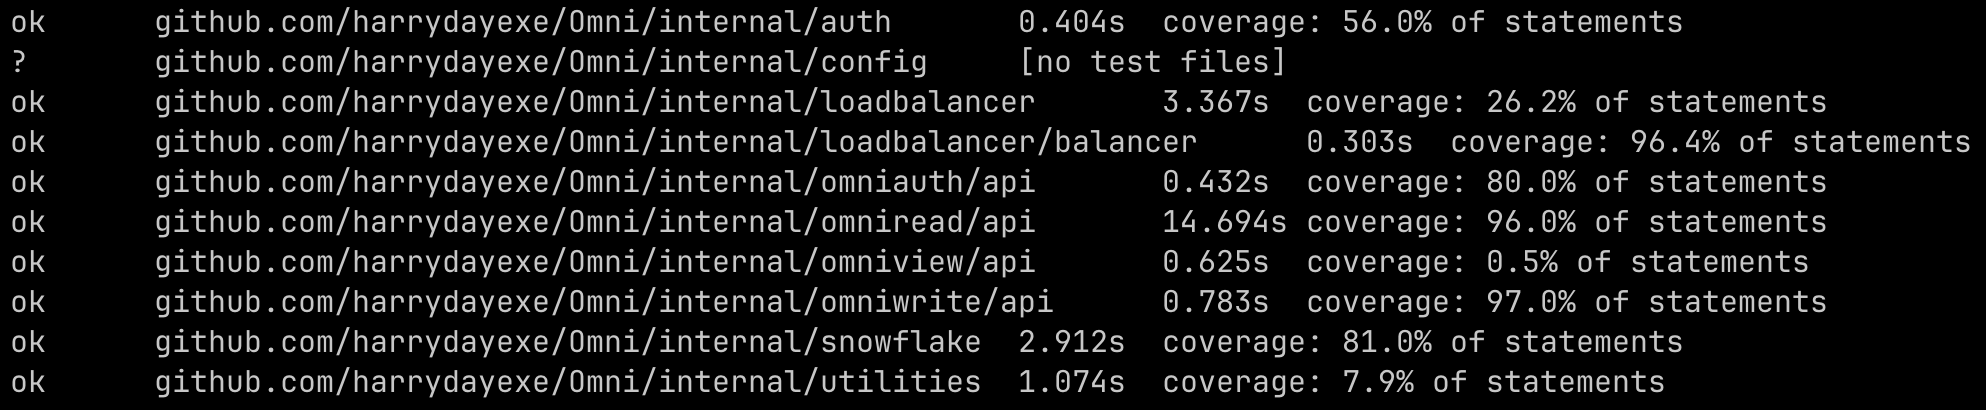
\includegraphics[width=12cm]{test-coverage.png}
\centering
\caption{Omni Test Coverage Report}
\label{fig:test-coverage}
\end{figure}

Demanding code coverage requirements (such as enforcing all code to be at least 70\% covered) is less effective and even detrimental to the actual defect rates of codebases.
Instead, it is more effective to encourage practitioners to focus on more in-depth code coverage metrics such as Modified Condition-Decision (MC/DC) coverage, which is much more effective at highlighting faults before they become user-facing errors \citep{hemmati2015effective}. 

\section{Integration Testing}
The second important aspect of testing is the use of integration tests. Unit tests, whilst powerful and robust, are inherently limited in scope.
To keep them self-contained and fast to execute, they should not interact with external services such as databases or APIs. This limitation is where integration tests shine.

As the name implies, the design of an integration test allows them to test how different sections (or units) of the system integrate.
Integration can include how an application interacts with a real database or external API.
Integration tests do not have the same expectations about runtime and, in some cases, can take minutes or even hours to execute more complex scenarios.
However, they should still enforce the same requirements around repeatability and reusability, again to build up a suite of test cases for a product to pass before an update ships to market. 

Whereas unit tests should be run consistently by the engineer throughout the development lifecycle, integration tests are usually only run after an engineer is confident in their work, often by a CI/CD tool.

\subsection{Testcontainers}
Engineers often face the challenge of ensuring that the integration tests they write are repeatable.
For example, a database needs to be reset to a common starting point before each run of the tests to ensure consistency across iterations. 

In 2015, an open-source project called \underline{\href{https://testcontainers.com}{Testcontainers}} \nocite{testcontainers} was released to the public, intending to solve just that issue.
Taking the example of an integration test that interacts with a database, instead of running the tests against a permanent database, which would need to be reset and modified after each run, the Testcontainers framework allows the creation of a database inside a container.
Each integration test can be run in parallel, connecting to different containers, ensuring that side effects from one test do not affect another. 

Because each test can define its dependencies in a container(s), the setup for each dependency is explicitly set in code and portable for any developer to run.
This allows integration tests to be run locally on an engineer's computer or in a larger CI/CD pipeline. 

Adopting Testcontainers for integration tests requires just a few lines of code to configure the container in each test case.
It brings all the benefits that ensure tests are repeatable, consistent and not flaky.

OmniRead utilises Testcontainers for integration testing between the request handlers and the underlying database logic, verifying that the queries written are accurate and valid.
A unit test cannot check the SQL queries themselves as the database layer is mocked to ensure speed when running the test suite.
Figure \ref{fig:testcontainers}\footnote{The ryuk container runs for the duration of the test suite and is responsible for killing any containers that are not terminated by the test suite itself (for example if one of the tests fails early)} shows the containers created as part of the integration test suite, demonstrating the parallelisation possible due to each test running on a fundamentally different database.

\begin{figure}[htbp]
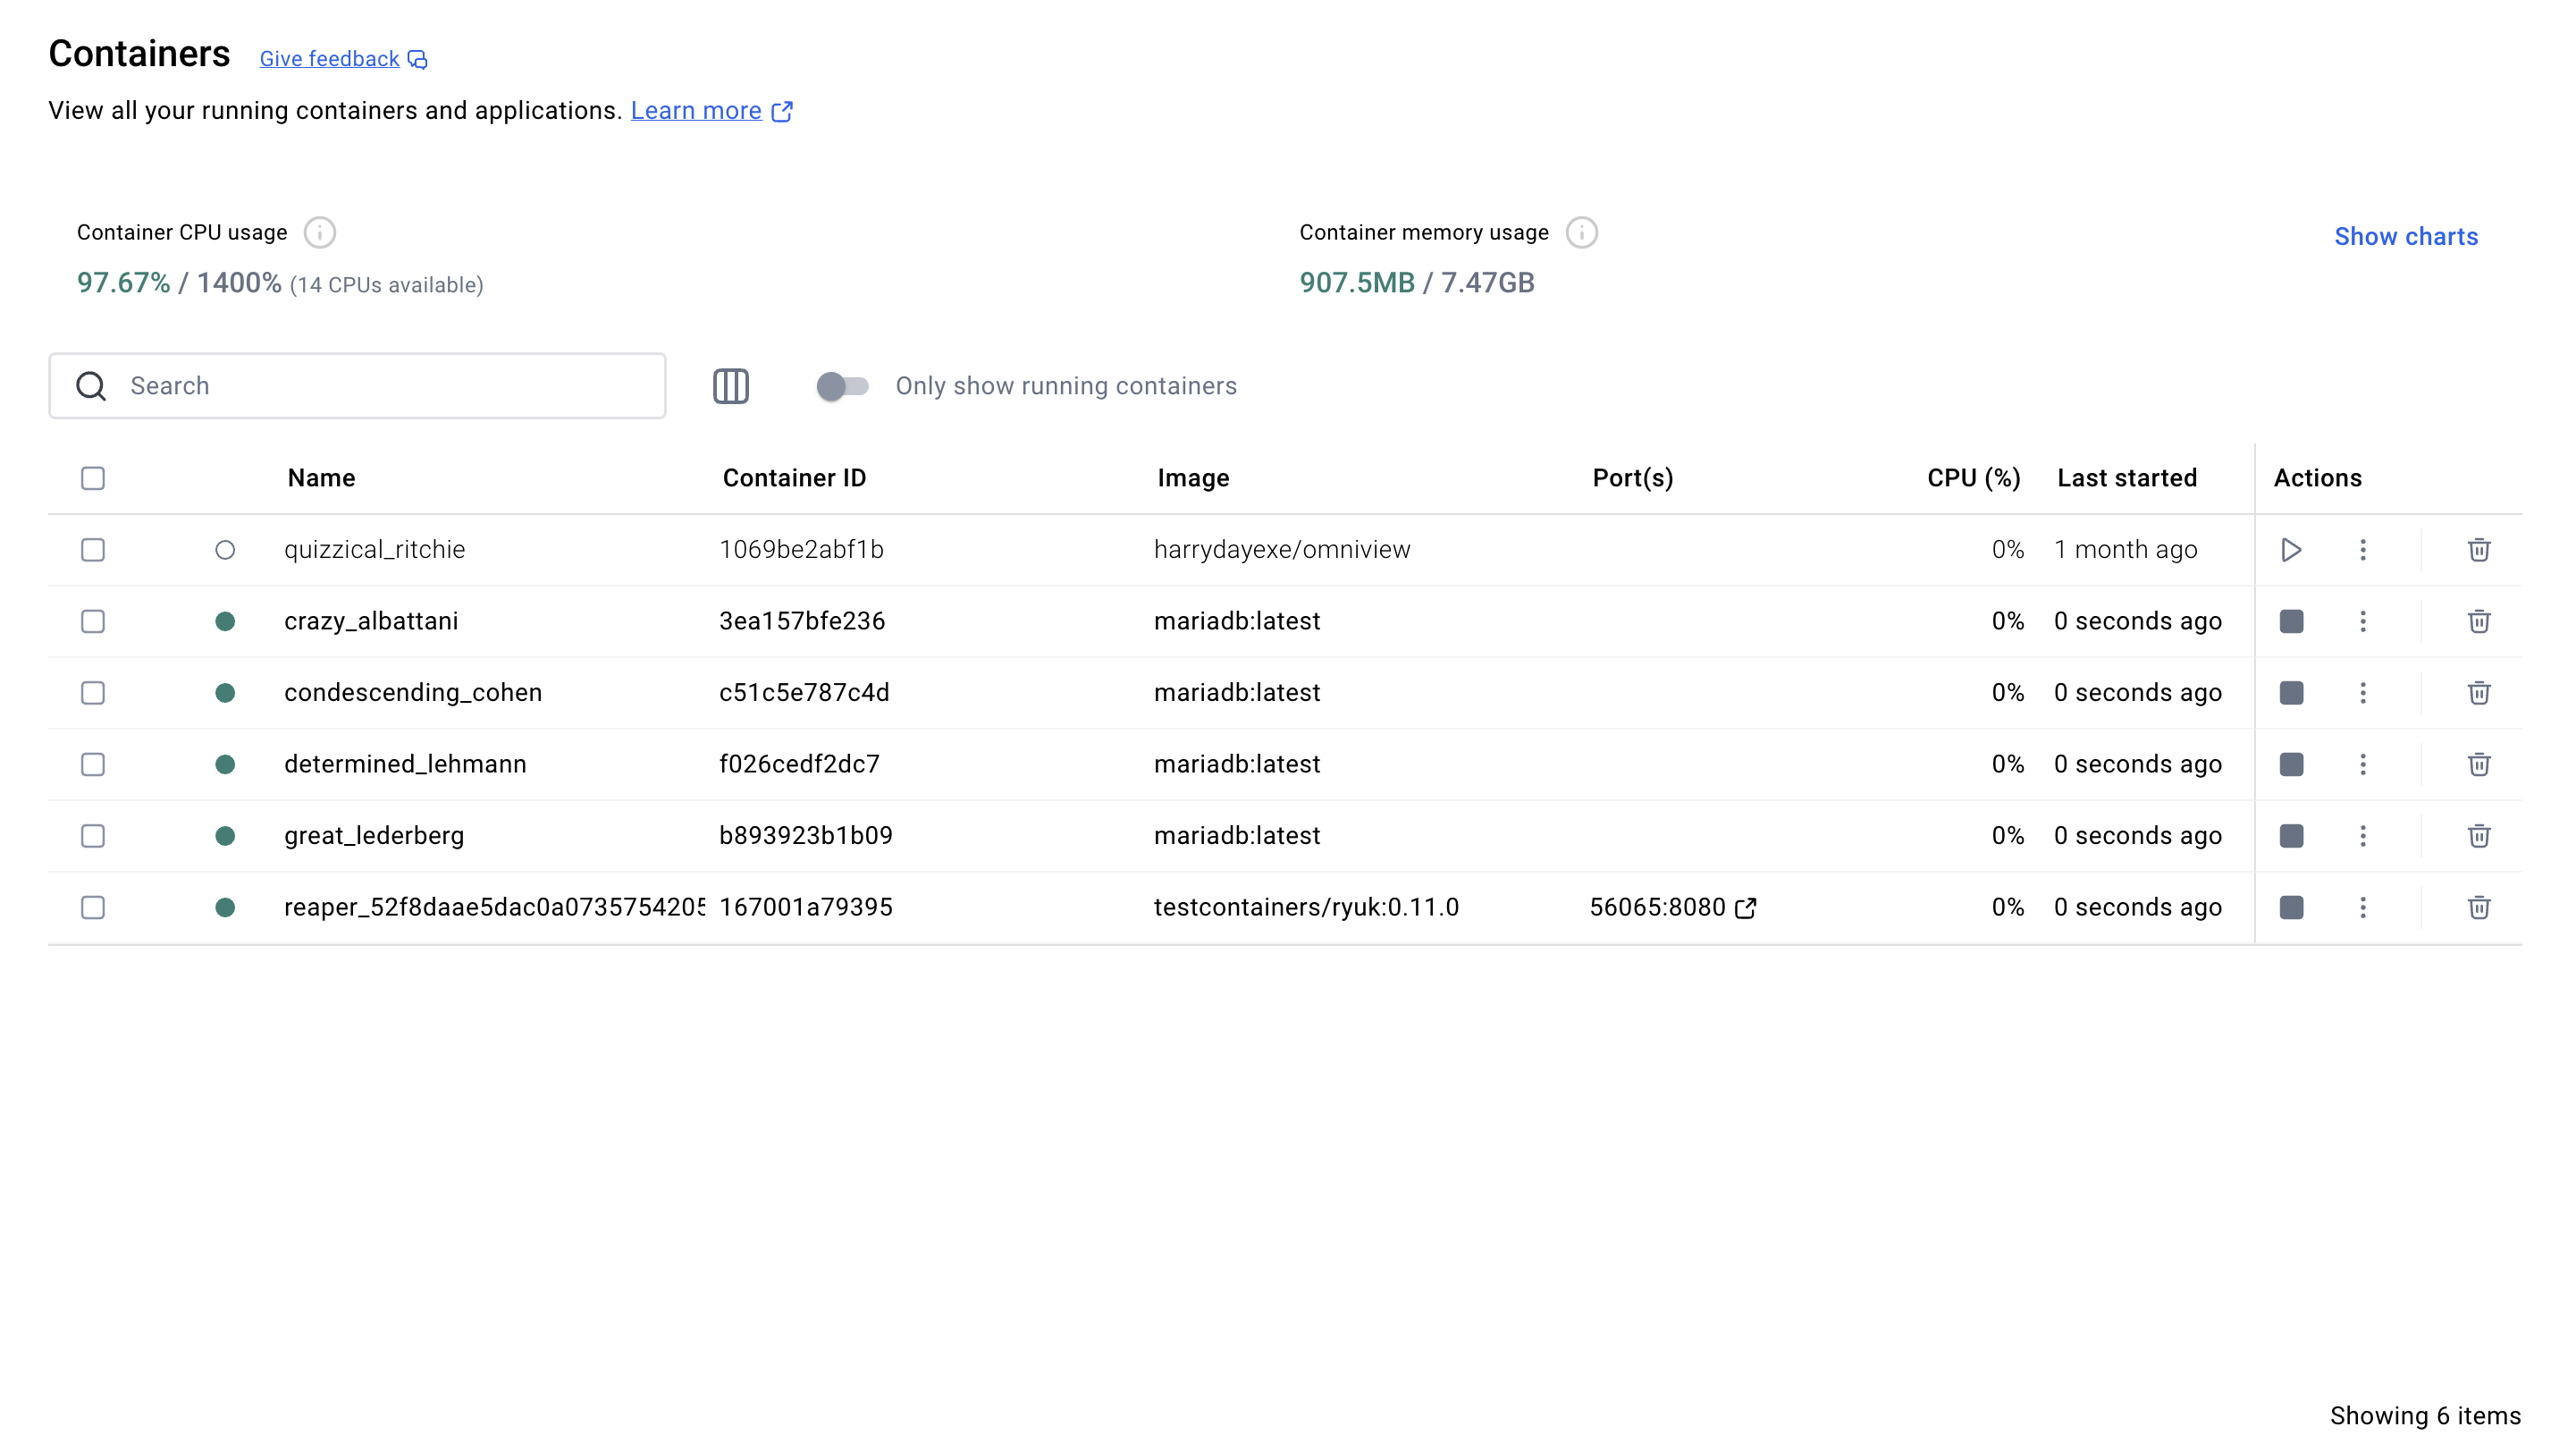
\includegraphics[width=12cm]{testcontainers.png}
\centering
\caption{Testcontainers Running during the Integration Tests}
\label{fig:testcontainers}
\end{figure}

\subsection{Testing of the Load Balancer}
Integration tests were needed to test the load balancers' ability to add and remove backends based on their health checks.
However Testcontainers also uses these health checks to ensure a container is ready before allowing a test to run.
In order to combat this, a custom health check container was built which exposes its actual health check on the non-standard endpoint \verb|testcontainersz|.
Using the non-standard endpoint allows the standard endpoints \verb|healthz|, \verb|livez|, and \verb|readyz| to be configured for testing purposes, precisely what is needed for the load balancer integration tests. 

The code for the health check tester application can be found at \underline{\href{https://github.com/harrydayexe/healthcheck-tester}{GitHub}} and the image is available on \underline{\href{https://hub.docker.com}{DockerHub}} for anyone to use.


\chapter{Reflection and Evaluation}
\label{cha:evaluation}

% TODO Complete the reflection and evaluation
Lorem ipsum dolar


% Bibliography
\bibliographystyle{agsm}
\bibliography{references}

% Appendices (if necessary)
\appendix
\label{sec:appendix}

\chapter{Middleware Implementations}
\label{sec:apdx-middleware-implementations}

\lstinputlisting[language=Go, caption={Logging Middleware Implementation}]{code-snippets/logging-middleware.go.bak}

\lstinputlisting[language=Go, caption={Max Bytes Middleware Implementation}]{code-snippets/max-bytes-middleware.go.bak}

\chapter{Screenshots of Frontend Design}
\label{sec:apdx-screenshots}

\begin{figure}[htbp]
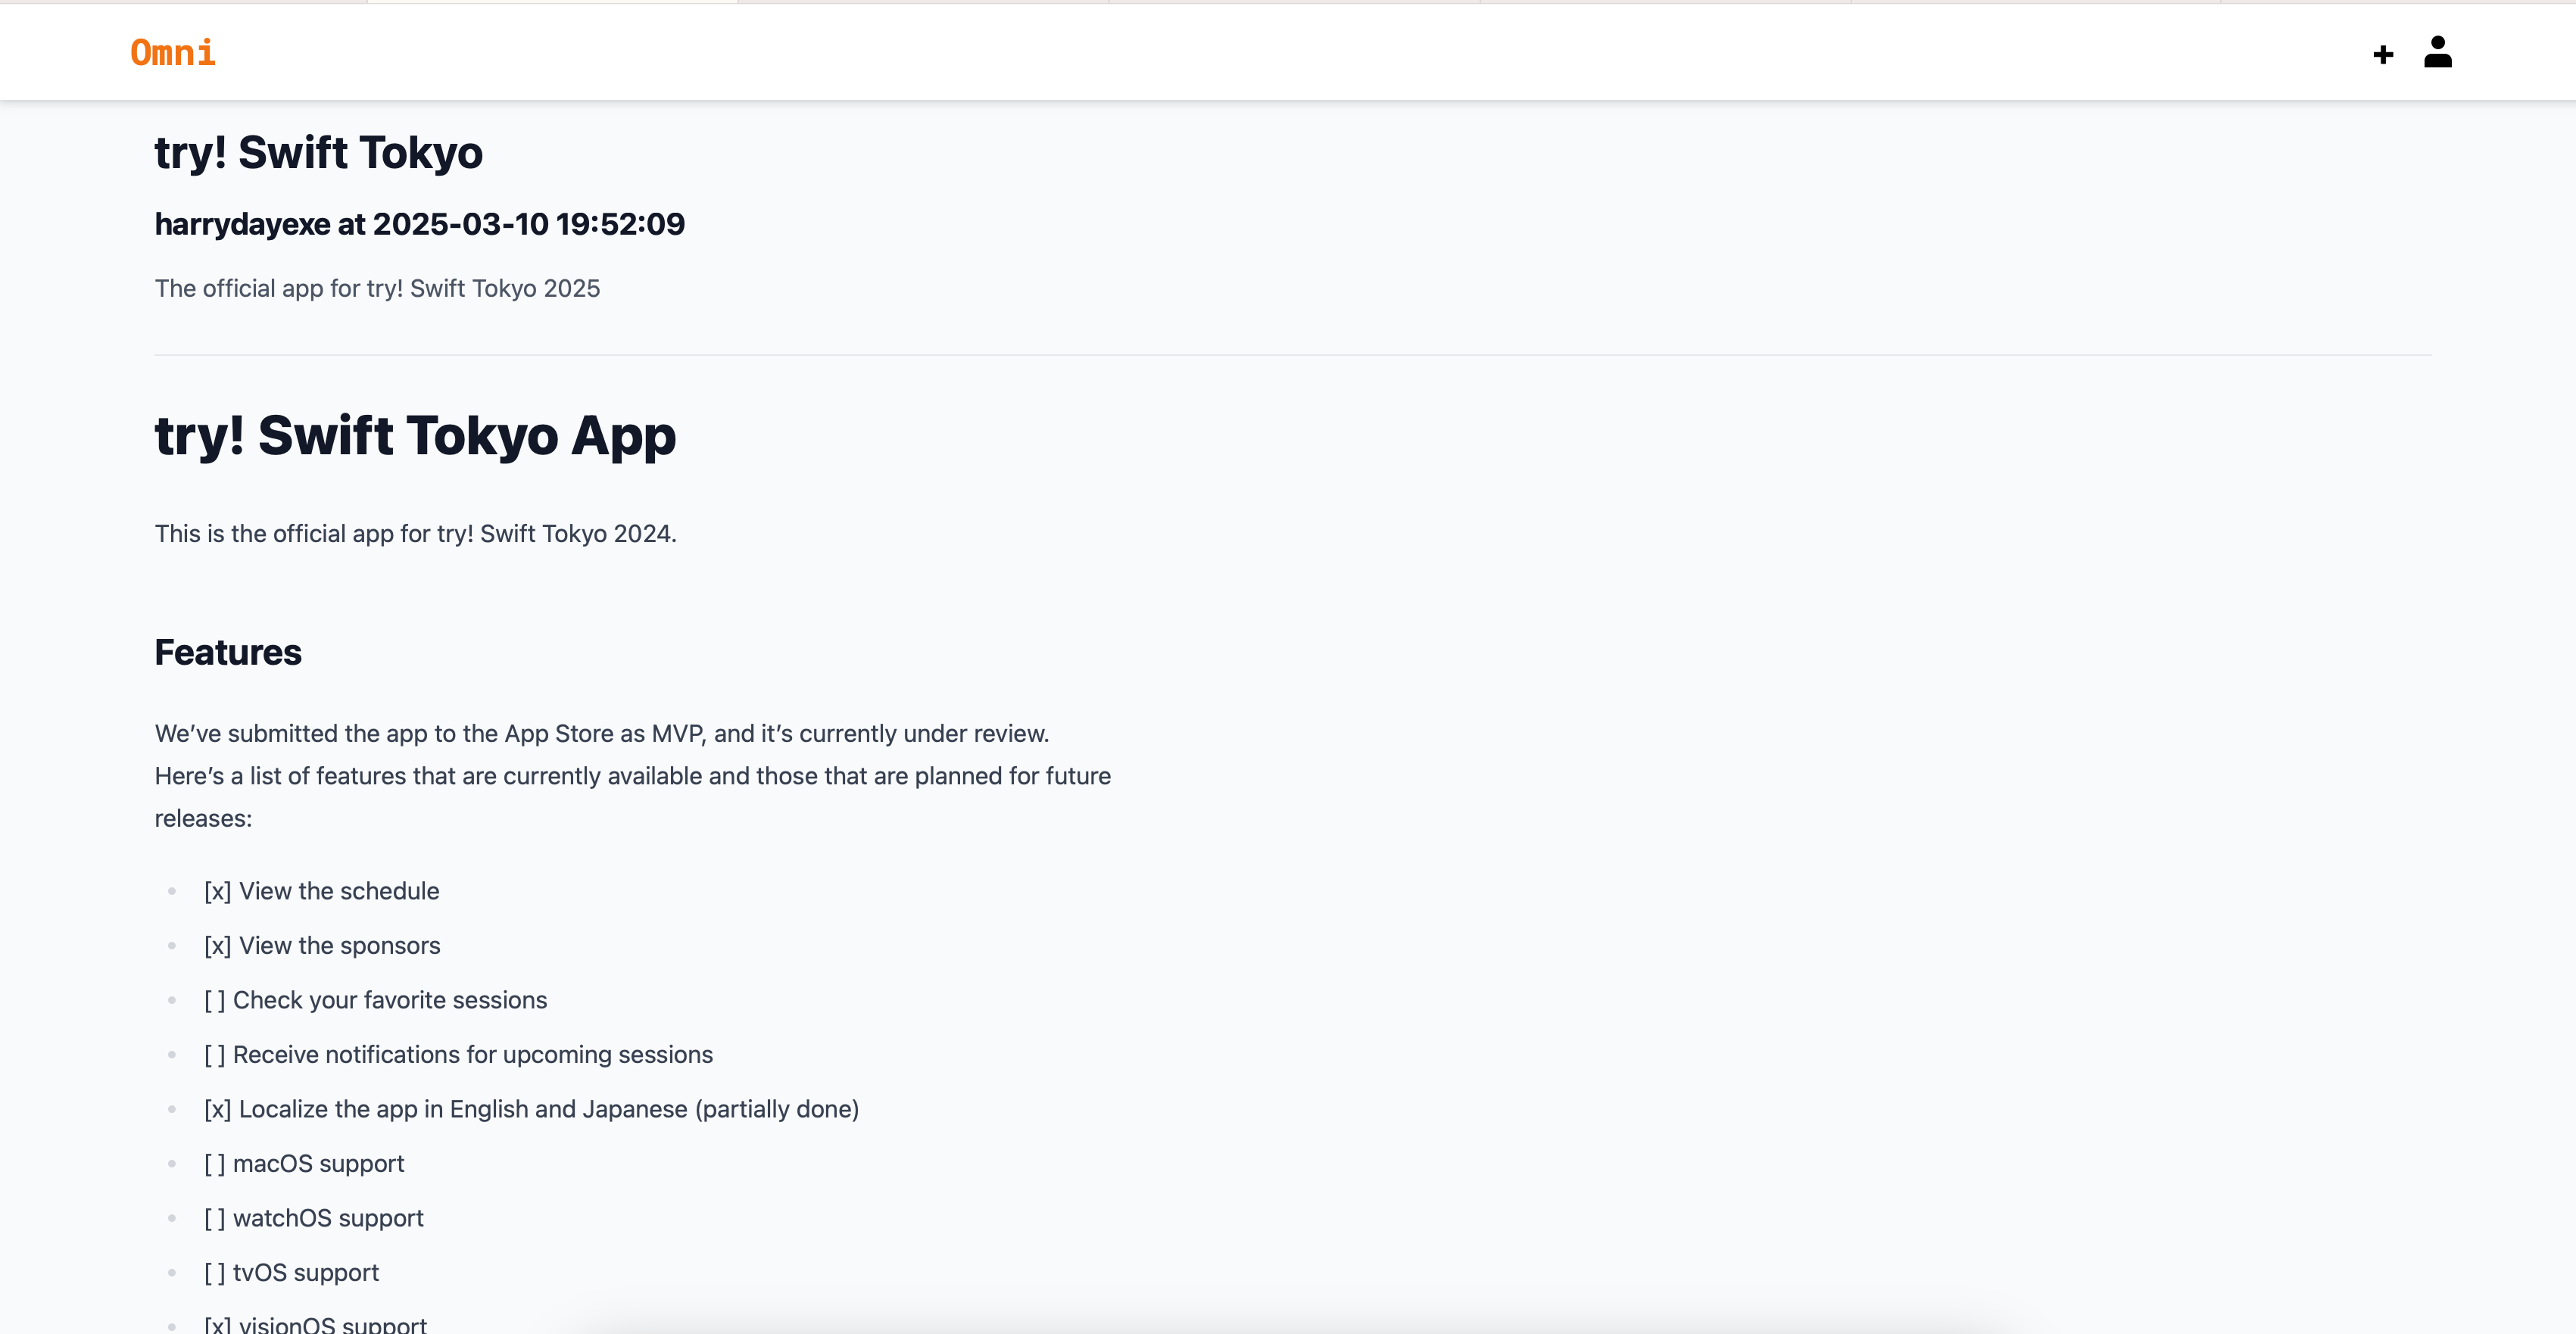
\includegraphics[width=12cm]{post-page-light.png}
\centering
\caption{Omni Post Page (Light Mode)}
\end{figure}

\begin{figure}[t]
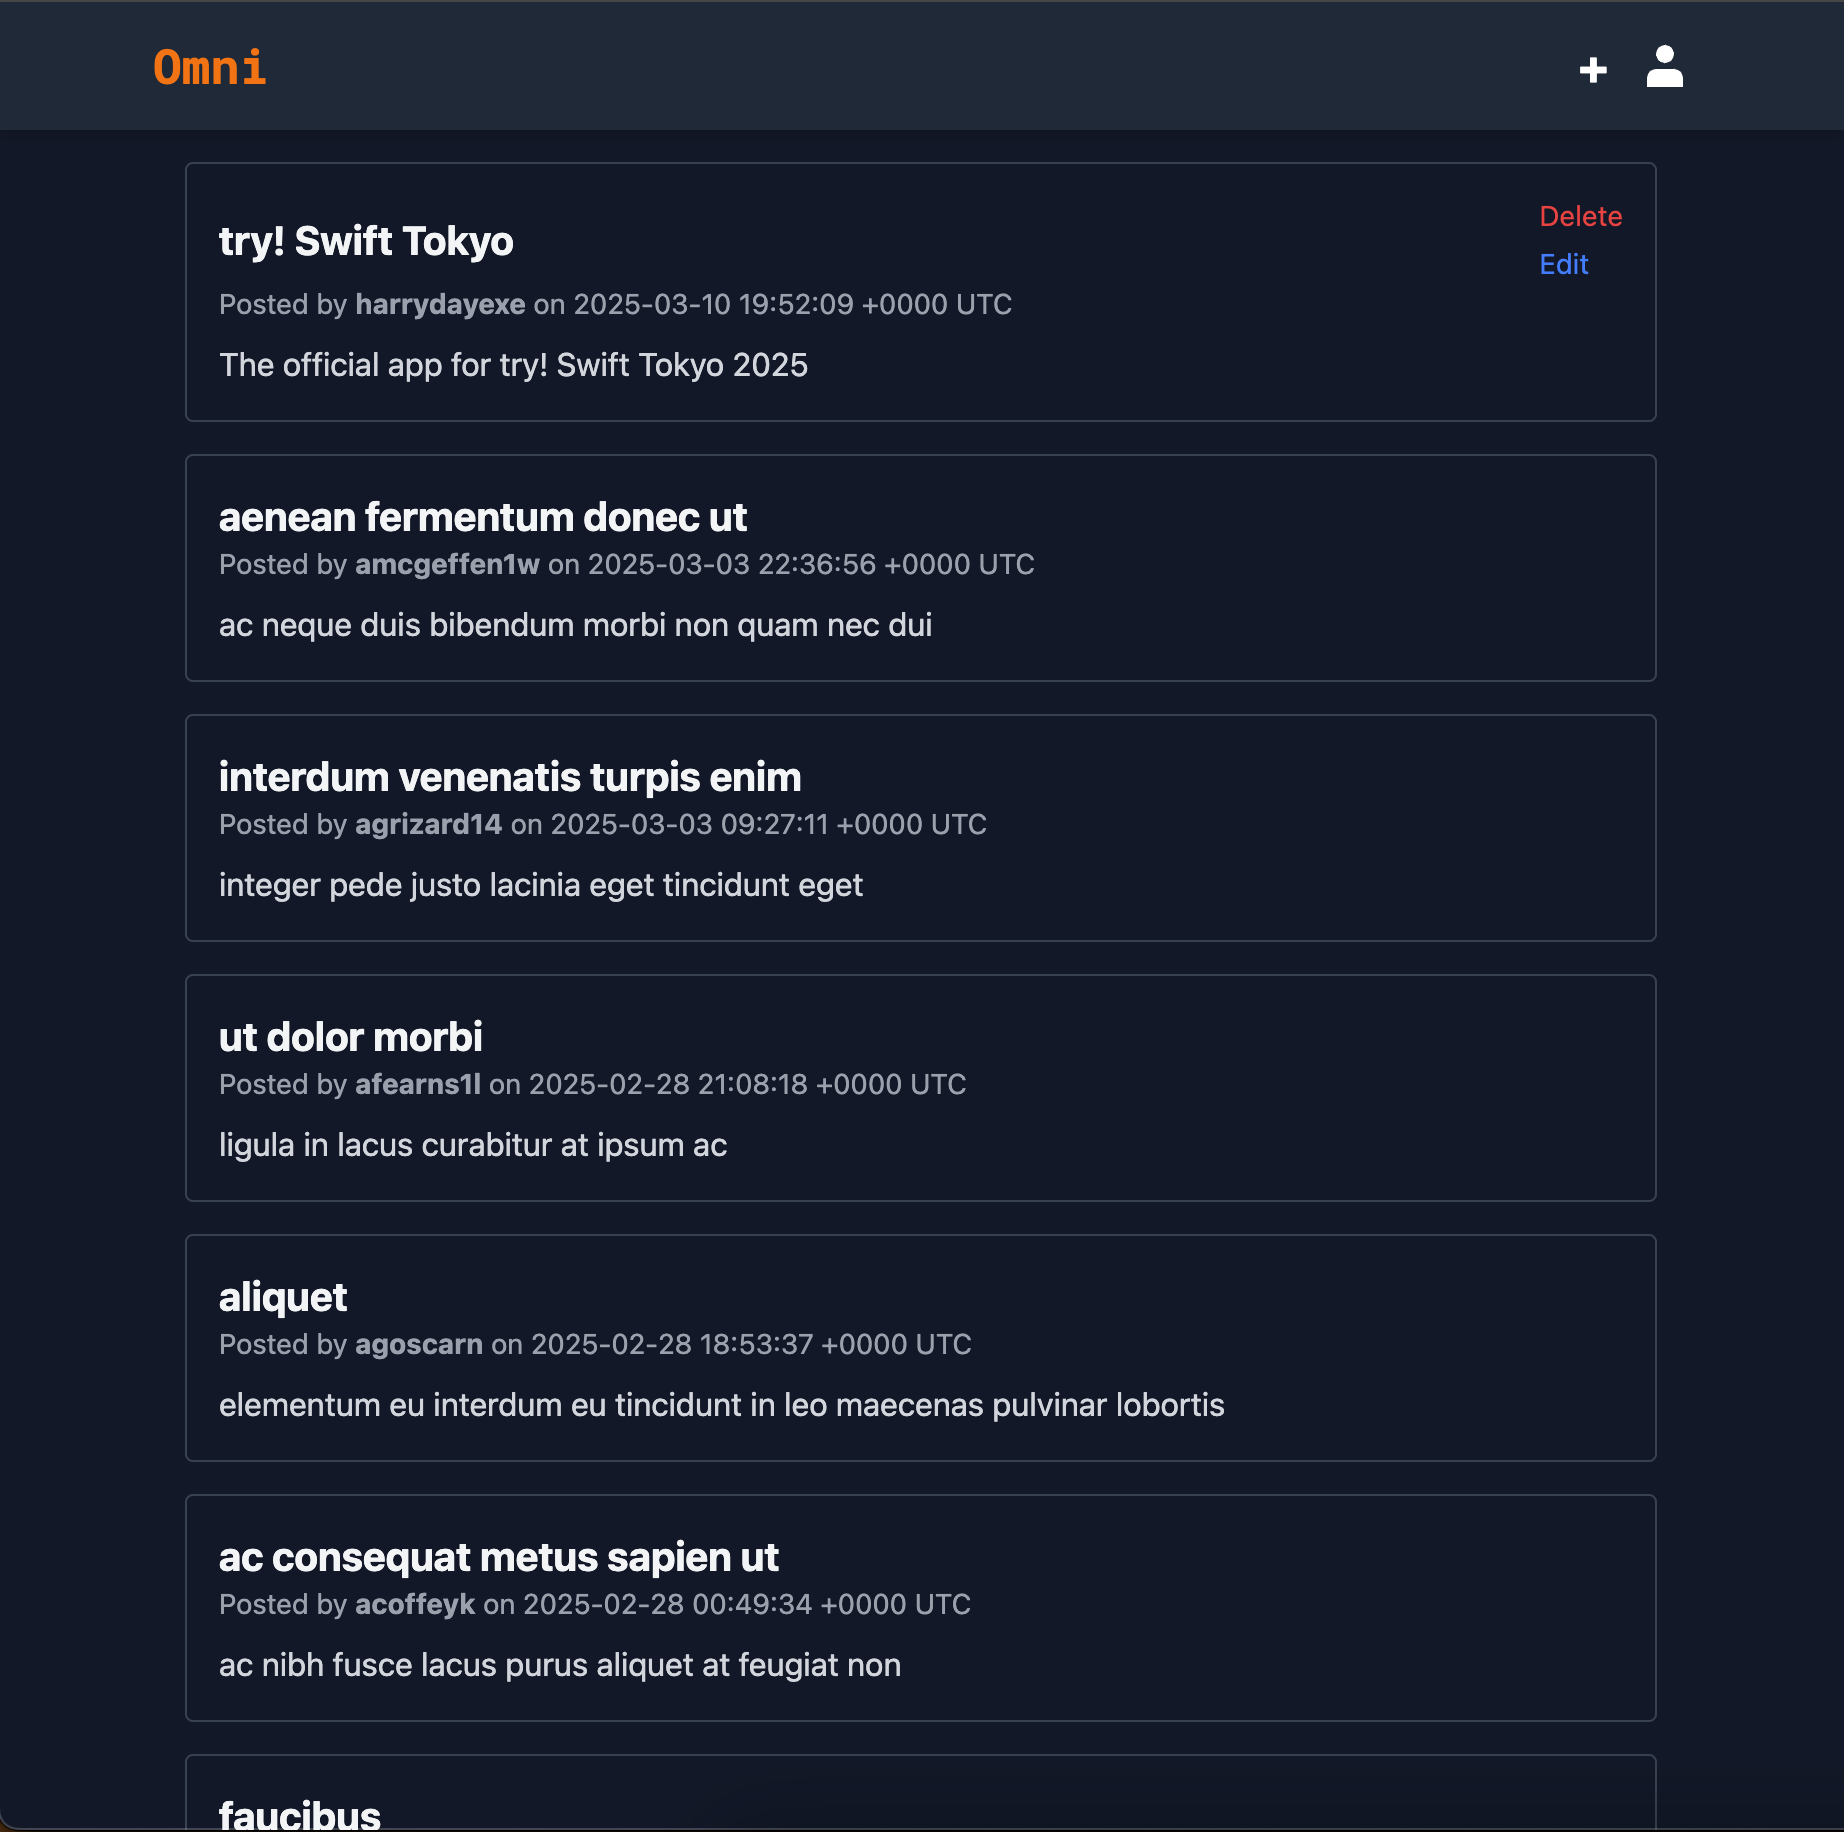
\includegraphics[height=9cm]{home-dark.png}
\centering
\caption{Omni Home Page (Dark Mode)}
\end{figure}

\begin{figure}[b]
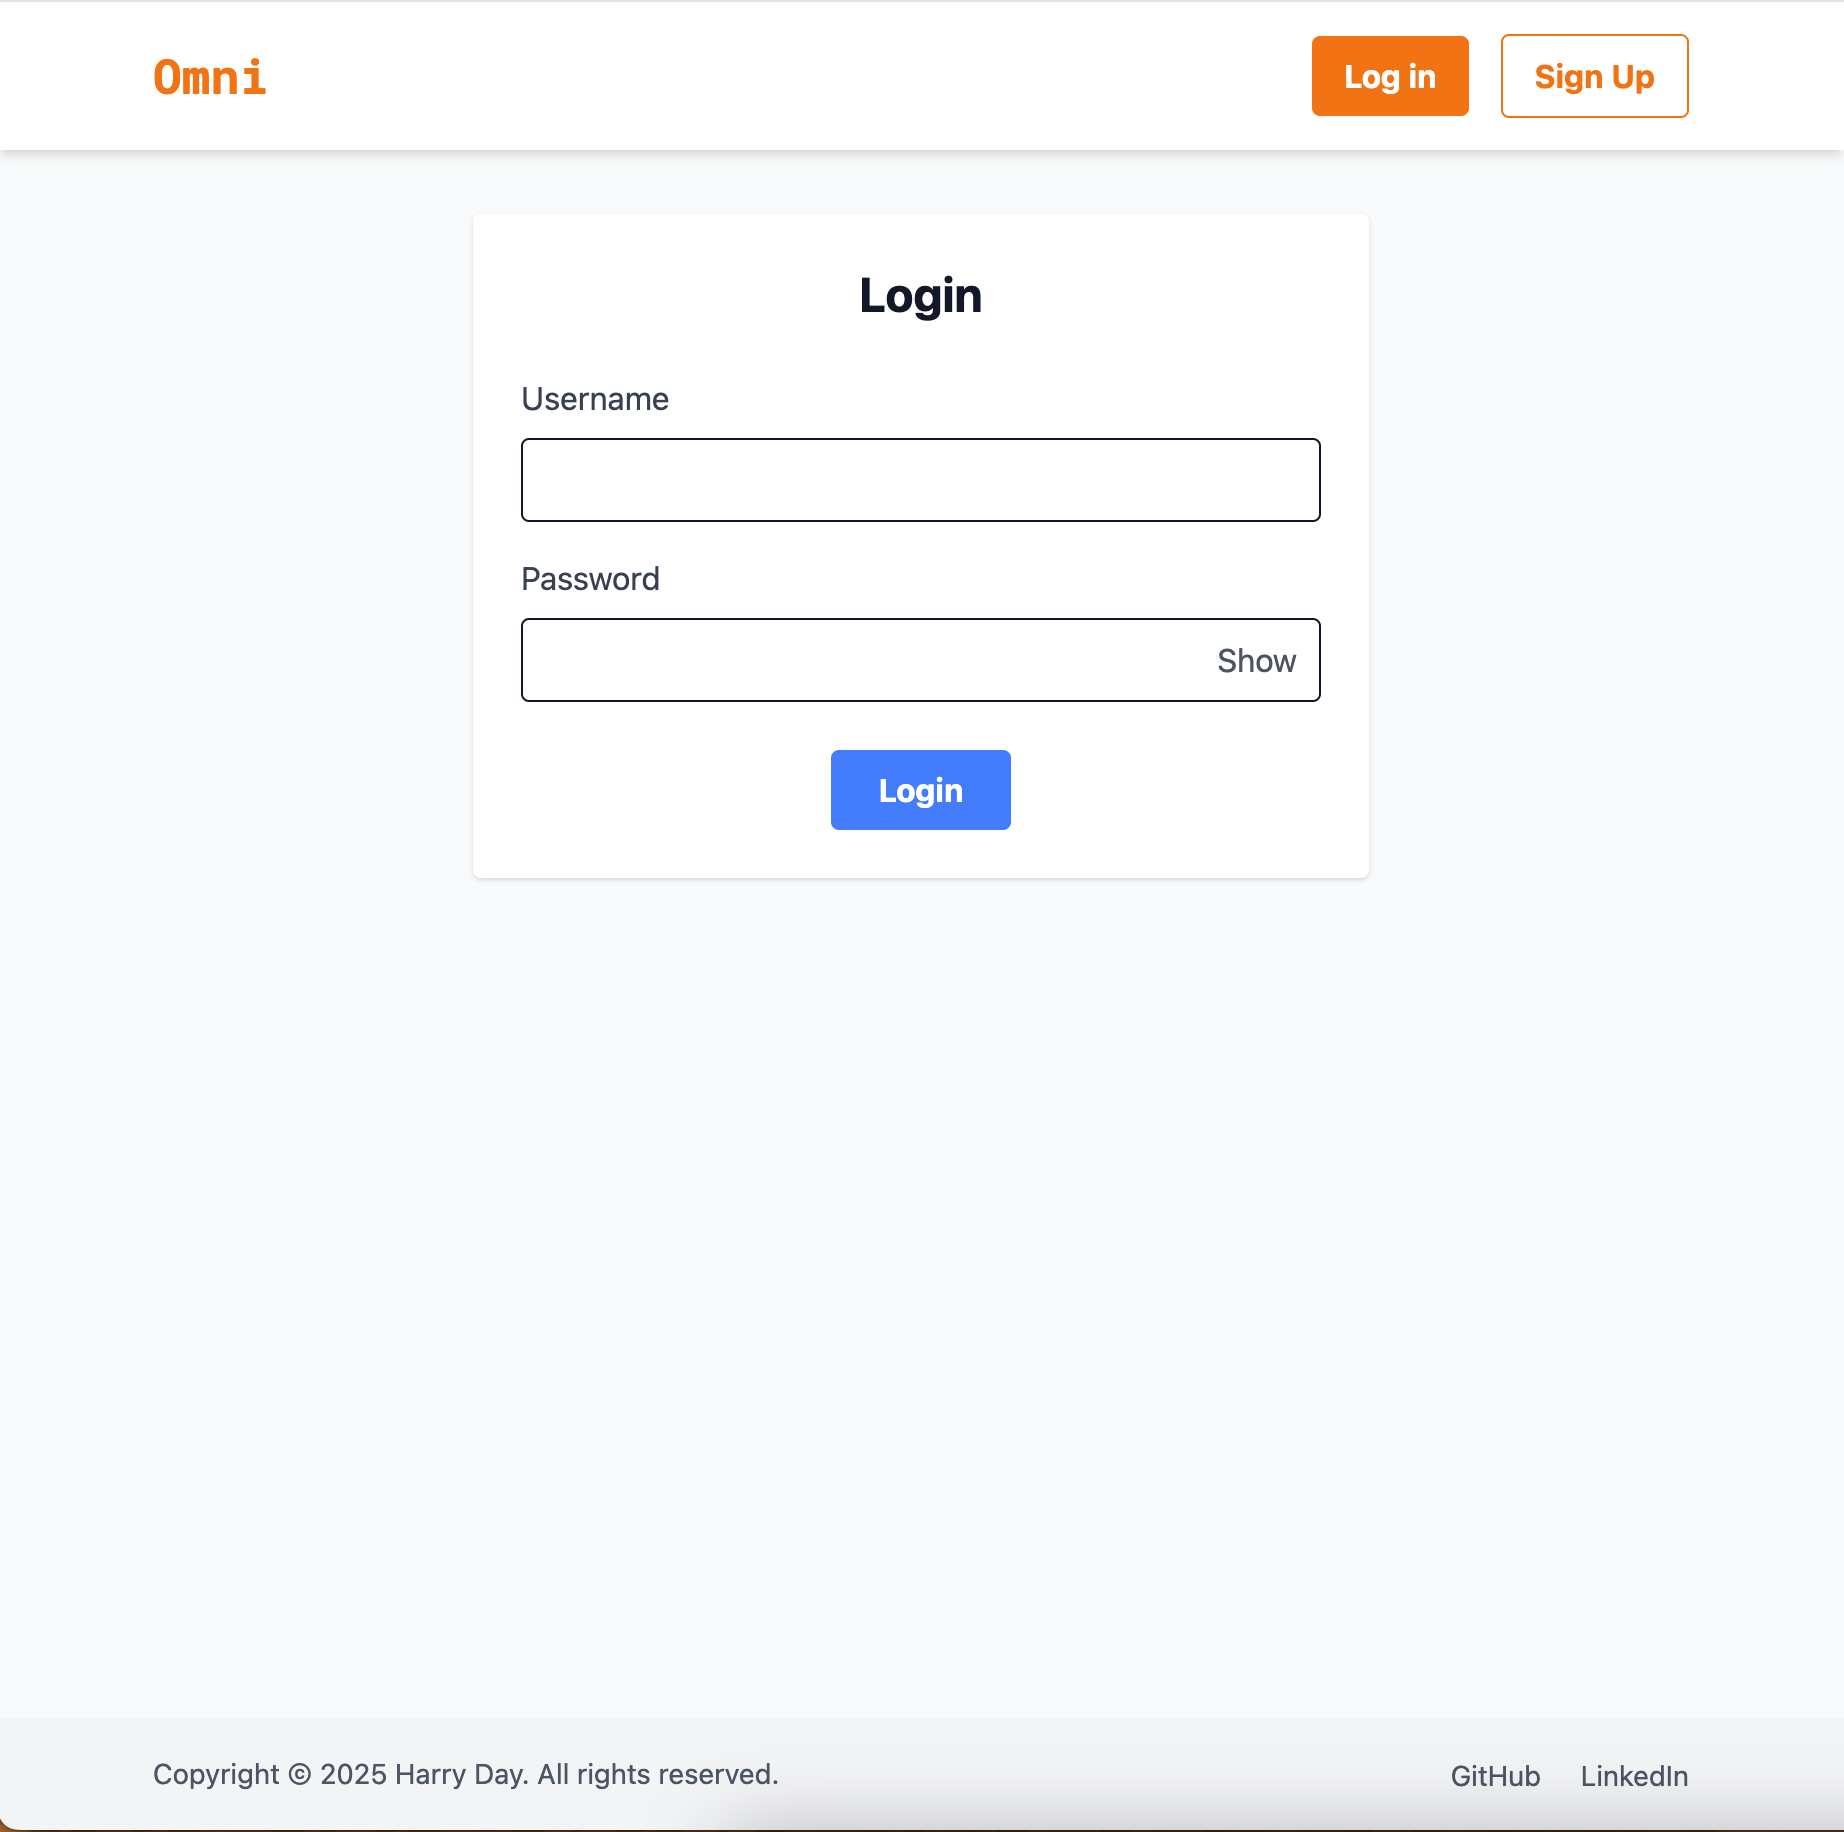
\includegraphics[height=9cm]{login-light.png}
\centering
\caption{Omni Login Page (Light Mode)}
\end{figure}

\begin{figure}[htbp]
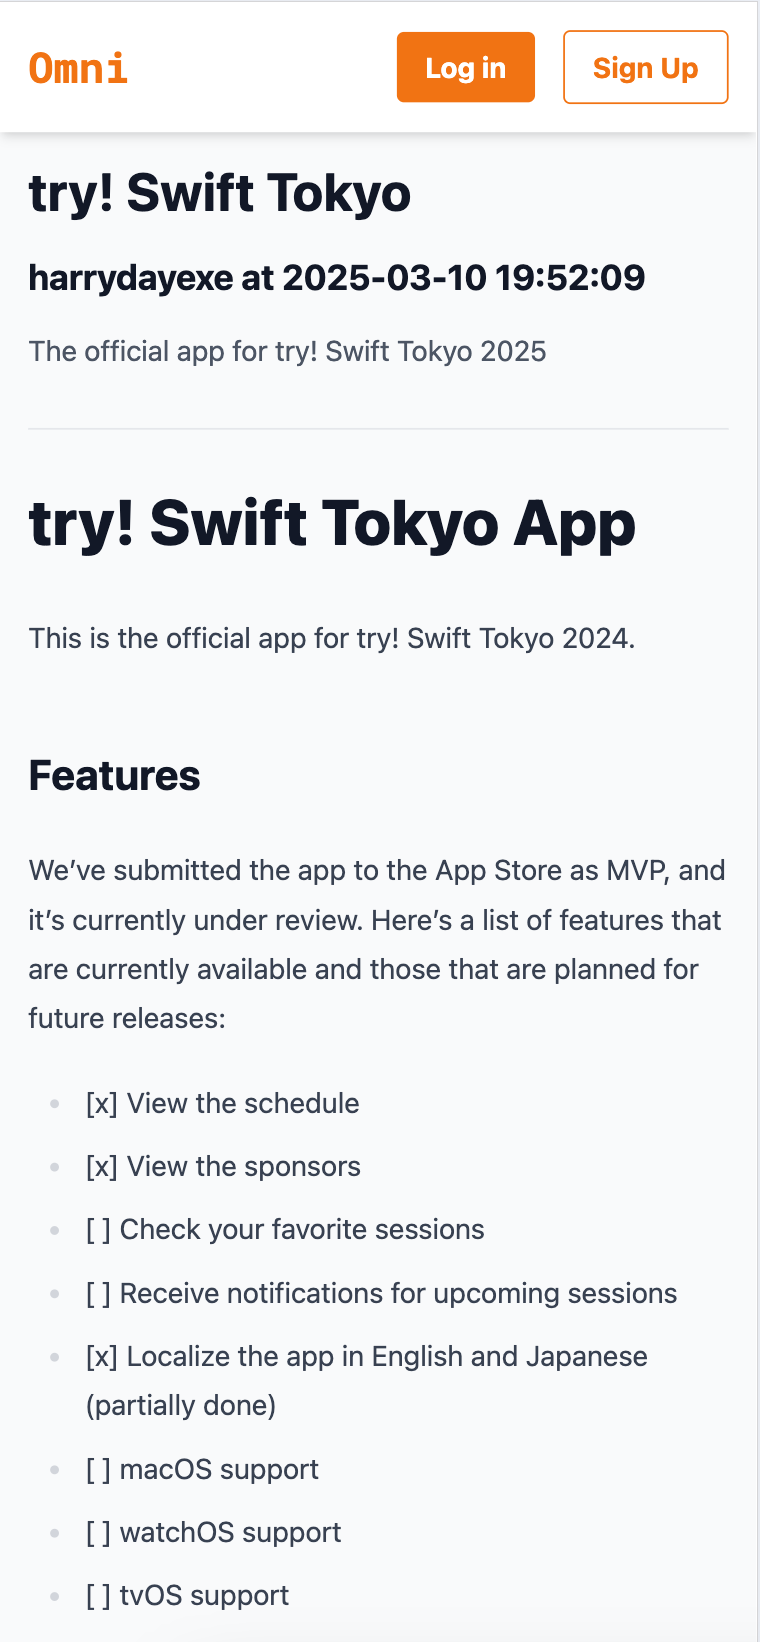
\includegraphics[height=12cm]{post-page-phone.png}
\centering
\caption{Omni Post Page (Mobile)}
\end{figure}

\chapter{Concurrency in OmniView}
\label{sec:apdx-concurrency-omni-view}

\lstinputlisting[language=Go, caption={Concurrency in OmniView}]{code-snippets/concurrency-support.go.bak}

\chapter{User Survey Responses}
\label{sec:apdx-user-survey}

\section{Questions}
\begin{itemize}
    \item How easy or difficult did you find the site to navigate? For example, when creating an account, viewing posts or writing a comment?
    \item Would the platform be helpful to you as a junior software engineer?
    \item Do you see yourself primarily producing or consuming content on Omni?
\end{itemize}

\section{Responses}

\subsection{Participant 1}
\subsubsection{Question 1}
Using Omni was a breeze! Everything went really well, from registering to responding to posts. I appreciated how easy the site was to navigate; I never got lost.

\subsubsection{Question 2}
Of course. It seems like a great place to learn and maintain ties with the tech community. It would be really beneficial for my development to have access to project ideas, industry discussions, and advice in one location.

\subsubsection{Question 3}
I would primarily be consuming content and learning at the moment. However, I'd love to eventually start sharing my own projects and advice as well.

\subsection{Participant 2}
\subsubsection{Question 1}
I found Omni to be very user-friendly. Whether I was reading posts or leaving comments, it was easy to find what I needed thanks to the simple design.

\subsubsection{Question 2}
Yes, absolutely! It appears to be a fantastic resource for both more complex subjects and advice aimed at beginners. I could see it greatly advancing my skill set.

\subsubsection{Question 3}
I'll primarily consume content to learn at first, but eventually I'd like to share interesting things I find or create tutorials.

\subsection{Participant 3}
\subsubsection{Question 1}
I had no trouble navigating Omni. The layout made it very easy to begin interacting, and creating an account was quick. It felt very natural to write comments and posts; the platform seems to be designed to make producing posts as simple as possible.

\subsubsection{Question 2}
Of course. Omni seems like the perfect platform for me to post tutorials, share my learning experiences, and even initiate conversations with other community members. Having a platform that makes contributing so easy and friendly is encouraging.

\subsubsection{Question 3}
Without a doubt, my primary goal is to produce content. I can't wait to share resources, write posts, and perhaps even document some of my ongoing projects. It seems like a wonderful place to learn and give back.

\subsection{Participant 4}
\subsubsection{Question 1}
The site follows the classic design conventions that social networks use, which assisted in finding the correct buttons and ui elements for creating an account and posting. 

\subsubsection{Question 2}
Yes, using the READMEs that I have already written for my projects is an innovative idea that reduces the barrier to producing content. However needing to find the link on GitHub to get the raw file was a little inconvenient. Maybe a future version could do this automatically. It makes it very easy to share my projects quickly.

\subsubsection{Question 3}
I would primarily be producing content to help my CV, but I would also be consuming content to get ideas from others. I think it is a great idea to have a platform that allows you to do both.



\end{document}
